\documentclass[handout]{beamer}

\usepackage{fontspec} 
% \usepackage{lsp-makros}
\useoutertheme{lsp}

\usepackage{lsptitle}
\usepackage[german]{babel}

\def\two@digits#1{\ifnum#1<10 0\fi\number#1}
\def\mytoday{\two@digits{\number\day}.\two@digits{\number\month}.\number\year}


\usepackage{xspace,multicol}
\newcommand{\latex}{\LaTeX\xspace}
\usepackage{tikz}


\newcounter{lastpagemainpart}
\footnotesep0pt
\renewcommand{\footnoterule}{}
\usefootnotetemplate{
  \noindent
  \insertfootnotemark\insertfootnotetext}

\let\beamerfn=\footnote
\renewcommand{\footnote}[1]{%
\let\oldfnsize=\footnotesize%
\let\footnotesize=\tiny%
\beamerfn<\thebeamerpauses->{#1}%
\let\footnotesize=\oldfnsize}


\date{\today}

\usepackage{eurosym}  
 
\renewcommand{\centerline}[1]{\hfill#1\hfill\hfill\mbox{}}


\title{Open Access in der\\ Sprachwissenschaft\medskip\\\Large Eine Disziplin stellt um.}
% \institute{FU Berlin}
\author[Nordhoff]{Sebastian Nordhoff}



\begin{document}
\lspbeamertitle


\frame{
\frametitle{Überblick}
%   \includegraphics[height=.2\textheight]{./path/to/graphicsfile}
  \tableofcontents
}
 
\section{Linguistik}
 \frame{
\frametitle{Linguistik}
%   \includegraphics[height=.2\textheight]{./path/to/graphicsfile}
  \begin{itemize}
       \item    25\,000 Linguisten
       \item        Abgrenzungsprobleme
       \item            Philologien
       \item            Sprachpädagogik
       \item        ungefähr genau so viele wie Teilchenphysiker
       \item    die naturwissenschaftlichtste utner den GW
       \item        englisch
       \item        Artikel
       \item        Peer Review
  \end{itemize}
}

\frame{
\frametitle{Sebastian Nordhoff}
%   \includegraphics[height=.2\textheight]{./path/to/graphicsfile}
  \begin{itemize}
    \item          Linguist
       \item        Paraguay
       \item        Sri Lanka
       \item    Entwickler
       \item        Glottolog-Datenbank mit 300.000 Referenzen und 27.000 Sprachen, Dialekte und Sprachfamilien
       \item    Open Everything activist
       \item    Geschäftsführer von Language Science Press
       \item    Mitarbeiter im Projekt KOALA bei der TIB

  \end{itemize}
}



\section[OA in der Linguistik]{Open Access in der Sprachwissenschaft}
\frame{
\frametitle{Open Access in der\\ Sprachwissenschaft}
  \bigskip
\includegraphics[height=.3\textheight]{glossa.png}\\~\\

  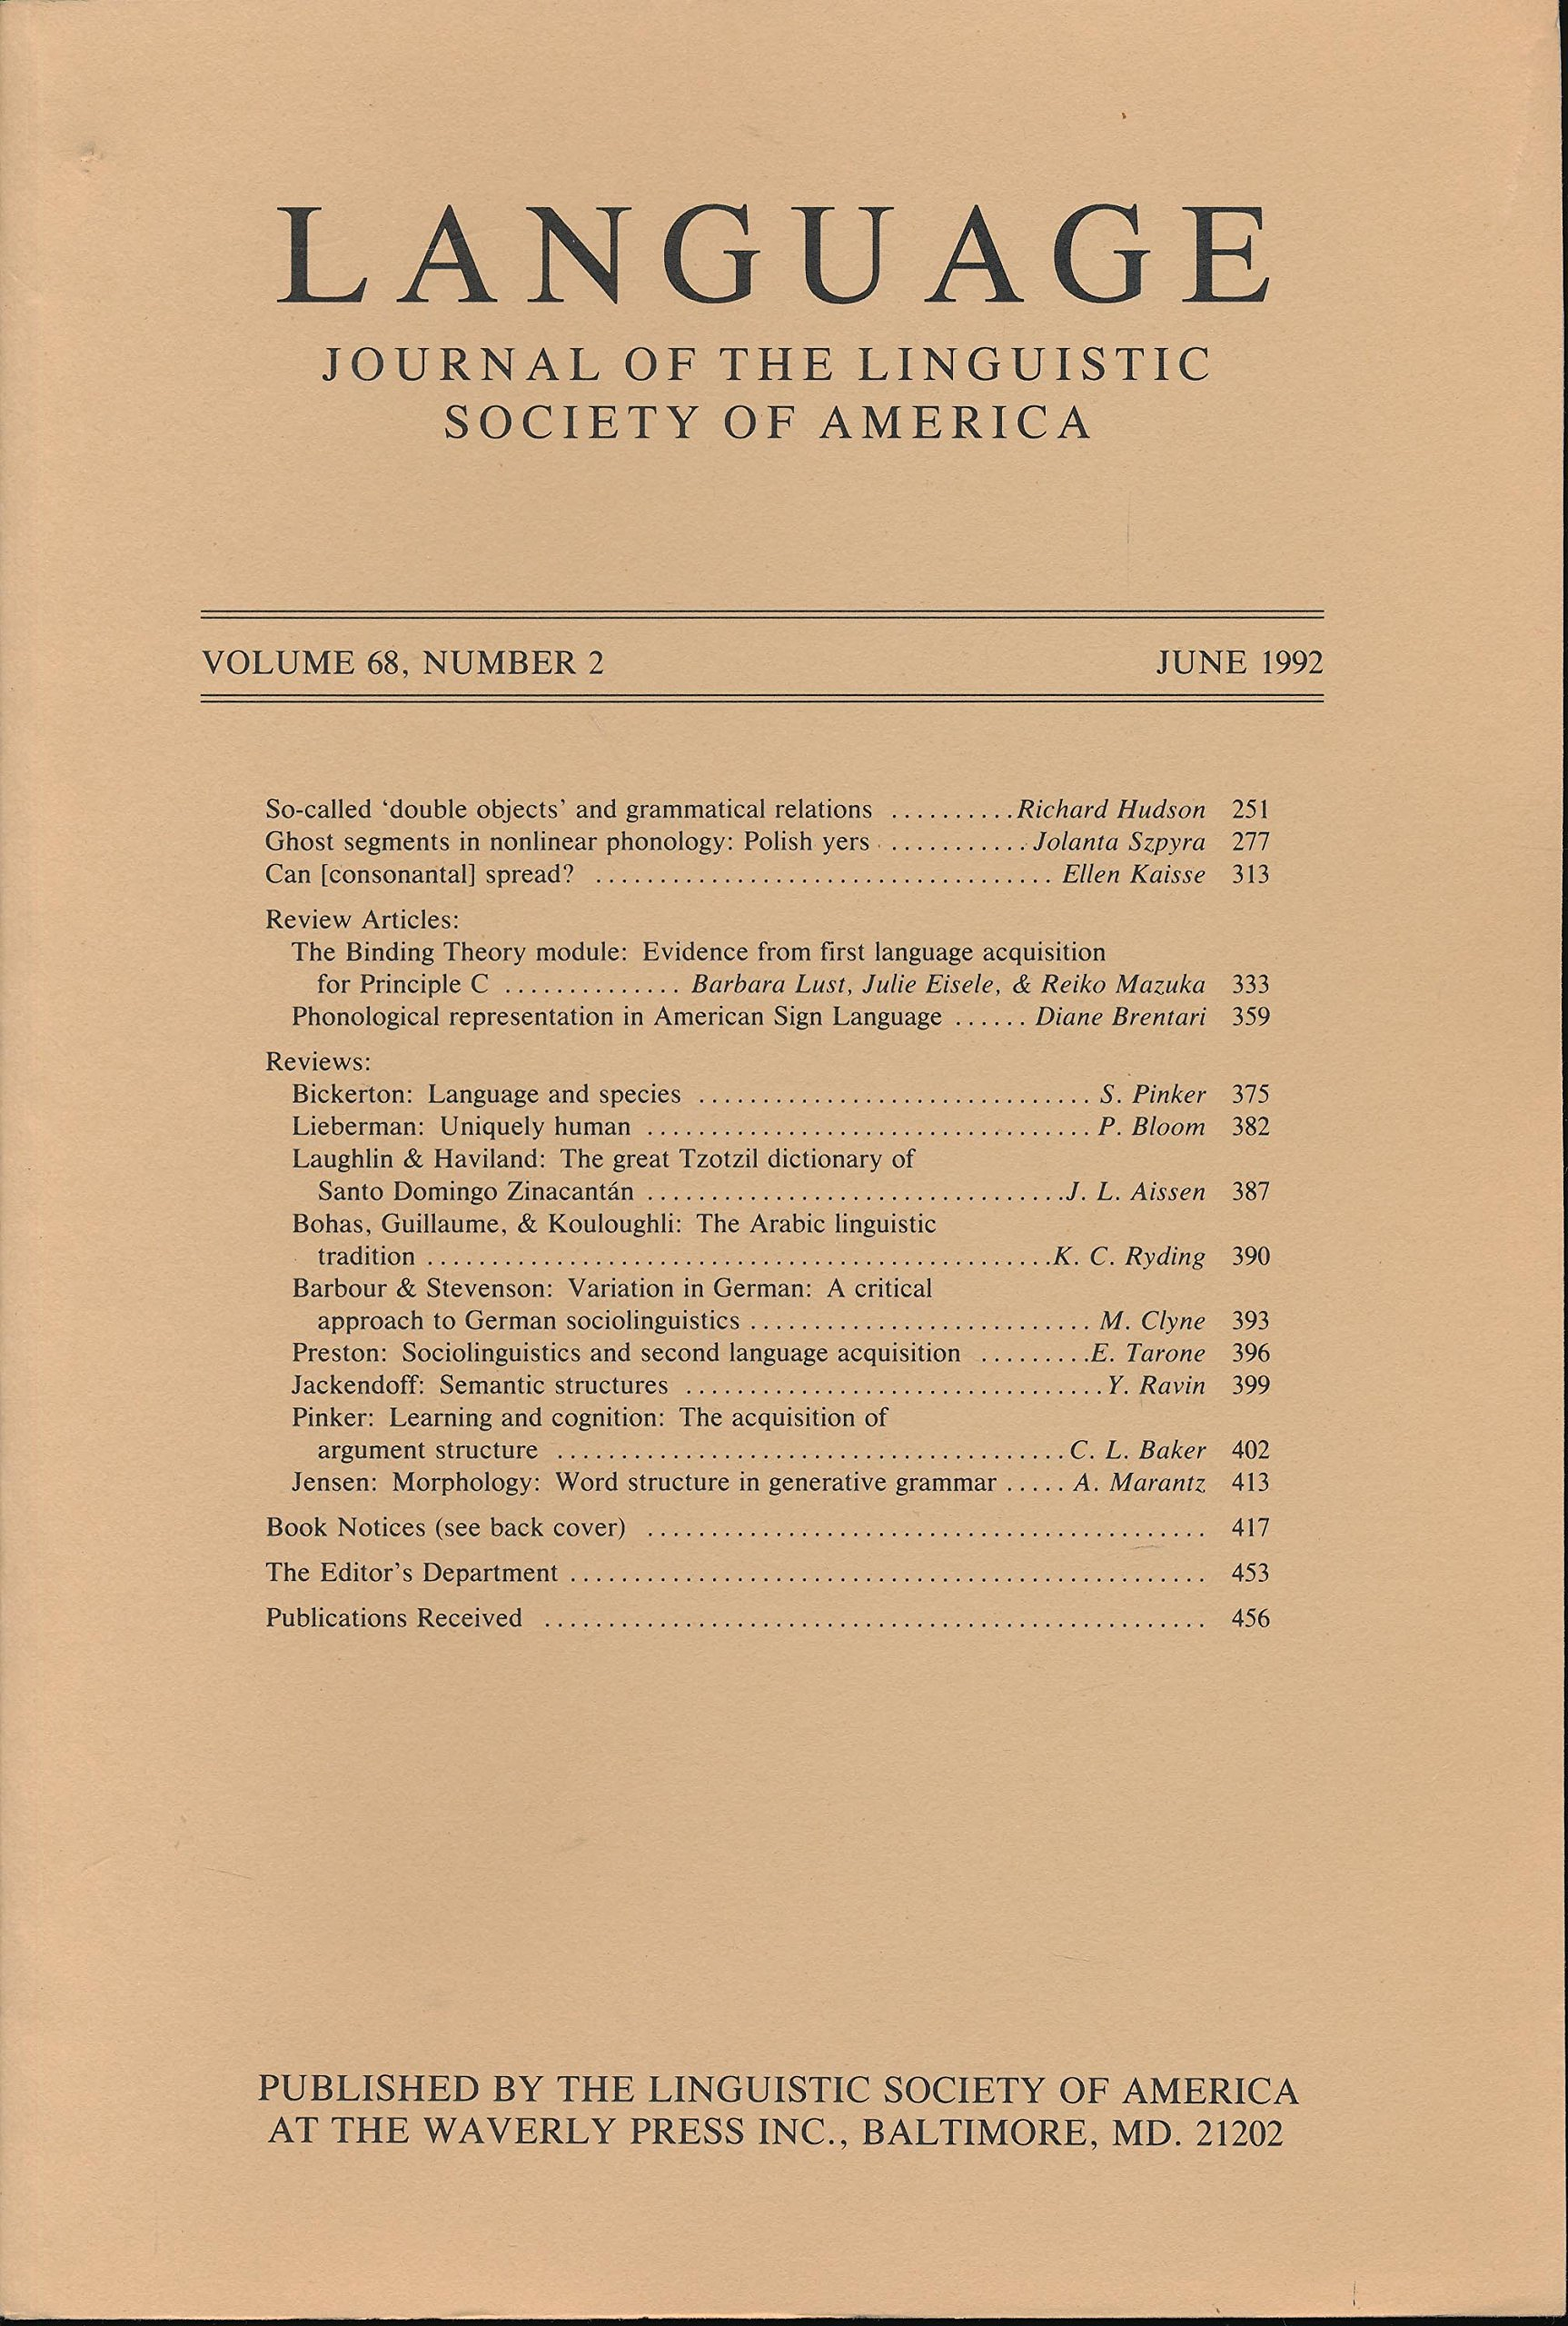
\includegraphics[height=.4\textheight]{language.jpg}
  
\includegraphics[height=.4\textheight]{zfs.jpg}
  
\includegraphics[height=.4\textheight]{langsci_logo_nocolor.pdf}

}

\subsection{Lingua/Glossa}
\frame{
\frametitle{Lingua/Glossa}
%   \includegraphics[height=.2\textheight]{./path/to/graphicsfile}
  \begin{itemize}
    \item         2015
       \item       \url{https://www.insidehighered.com/news/2015/11/02/editors-and-editorial-board-quit-top-linguistics-journal-protest-subscription-fees}
       \item       \url{https://www.heise.de/tp/news/Elsevier-Abtruennige-gruenden-neues-Open-Access-Journal-2912220.html}
       \item       \url{https://www.wired.com/2015/11/editors-of-the-journal-lingua-protest-quit-in-battle-for-open-access}
       \item   Herausgeber und Editorial Board fordern faire APCs
       \item    Elsevier ist zu keinen Zugeständnissen bereit
        Übergangsphase
  \end{itemize}
}



\frame{
\frametitle{Lingua/Glossa heute}
%   \includegraphics[height=.2\textheight]{./path/to/graphicsfile}
  \begin{itemize}
    \item           Glossa
        \begin{itemize}
                \item          2016--2021: 5,5 Jahre
                \item          700 Artikel
                \item              120 Artikel/Jahr
                \item          im großen und ganzen gleiche Autorenschaft wie vorher
        \end{itemize}
    \item      Zombie Lingua
        \begin{itemize}
        \item           2020: 102 Artikel
%         \item                  <https://www.sciencedirect.com/journal/lingua/vol/168/suppl/C>
%         \item                      <https://www.sciencedirect.com/journal/lingua/vol/244/suppl/C>
        \item          andere Autorenschaft
            \begin{itemize}
            \item              Ostasien
            \item              Arabische Welt
            \item              Iran
            \end{itemize}
        \end{itemize}
  \end{itemize}
}

\frame{
\frametitle{Lingua 170 (2016) vs.\\ Lingua 258 (2021)}
\hfill
  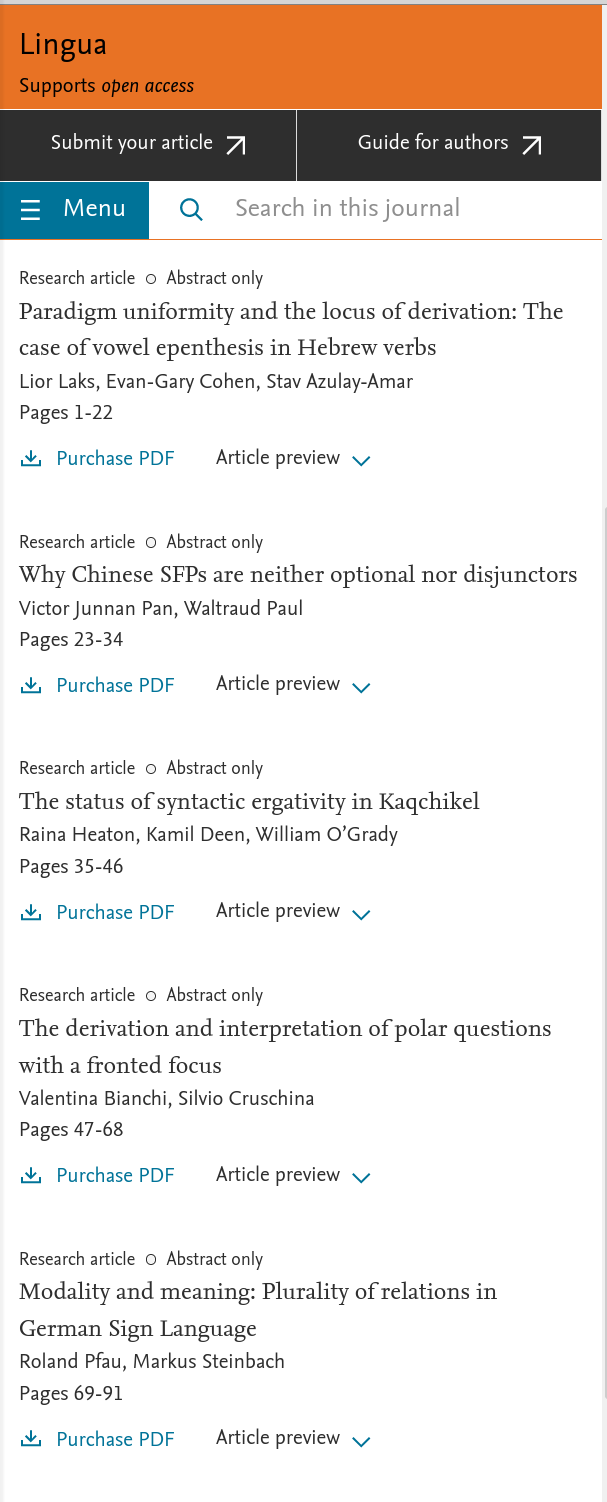
\includegraphics[height=\textheight]{lingua-alt.png}
  \hfill
  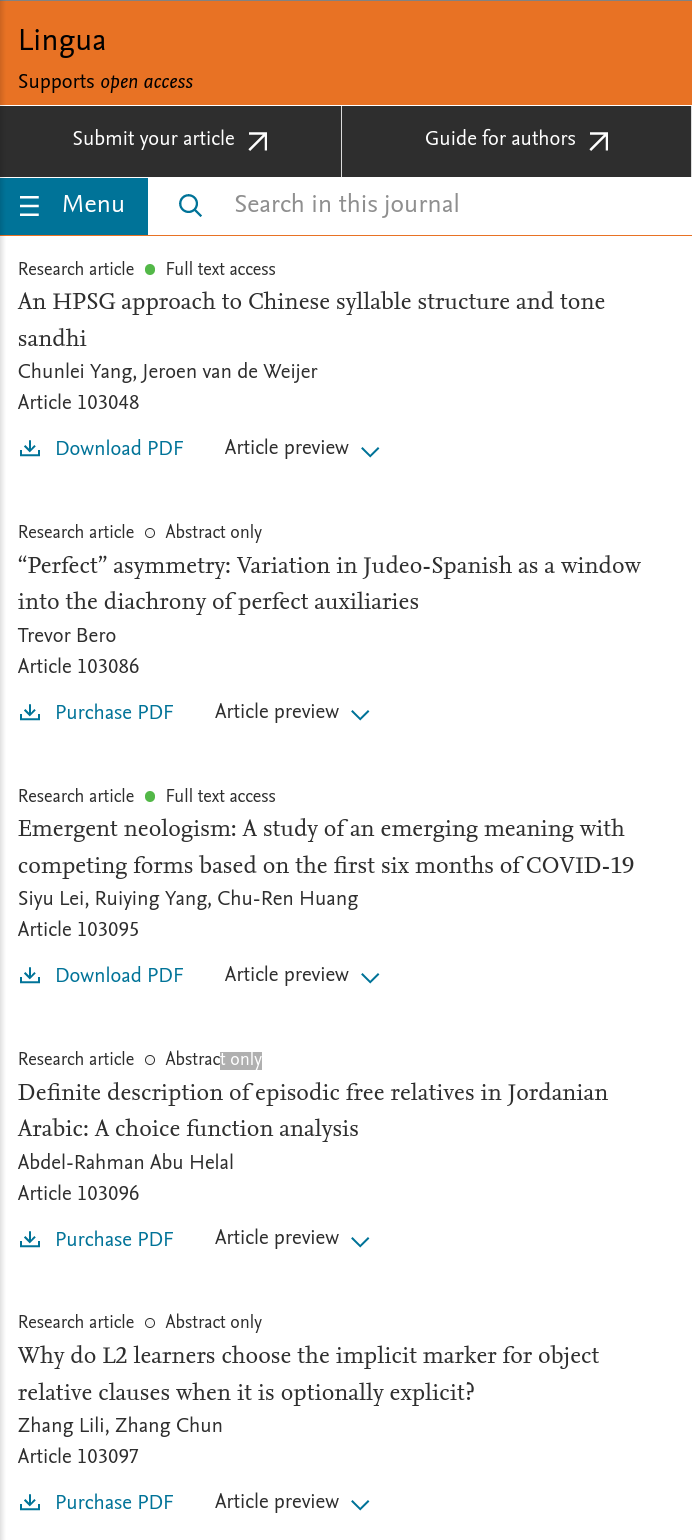
\includegraphics[height=\textheight]{lingua-neu.png}
  \hfill~
}


 \frame{
\frametitle{LingOA}
%   \includegraphics[height=.2\textheight]{./path/to/graphicsfile}
{\small
LingOA will provide a framework for the smooth transition from the traditional journal subscription model to Fair Open Access publishing. LingOA aims at developing an affordable and sustainable business model for Open Access publishing.

Several leading, international linguistics journals are being transferred from their current traditional publisher to a new Open Access publisher. This open access publisher complies with the following conditions:
}

\begin{enumerate}
  \item  The editorial board owns the title of the journals.
  \item  The author owns the copyright of his articles, and a CC-BY license applies.
  \item  All articles are published in Full Open Access (no subscriptions, no ‘double dipping’).
  \item  Article processing charges (APCs) are low (around 400 euros),  transparent, and in proportion to the work carried out by the publisher.
\end{enumerate}


}

\frame{
\frametitle{LingOA}
\begin{columns}
  \column{6cm}

  \begin{itemize}
        \item Glossa
       \item        Laboratory Phonology
       \item        Journal of Portuguese Linguistics
       \item        Italian Journal of Linguistics
  \end{itemize}
  \column{4cm}\centering
  
\includegraphics[width=4cm]{rooryck.png}\\Johan Rooryck
  \end{columns}
}


\subsection{Zeitschrift \glqq Language\grqq}
\frame{
\frametitle{Zeitschrift \glqq Language\grqq}
%   \includegraphics[height=.2\textheight]{./path/to/graphicsfile}
  \begin{itemize}
       \item    Referenz-Zeitschrift in der Linguistik
       \item    gehört der Linguistic Society of America
       \item    12 Monate Embargo, danach freier Zugriff
       \pause
       \item    mentimeter
       \pause
       \item    400 EUR APCs
  \end{itemize}
}


\subsection{Zeitschrift für Sprachwissenschaft}
\frame{
\frametitle{Zeitschrift für\\ Sprachwissenschaft}
%   \includegraphics[height=.2\textheight]{./path/to/graphicsfile}
  \begin{itemize}
     \item    Zeitschrift der deutschen Gesellschaft für Sprachwissenschaft
     \item    historisch hybrid mit APCs
     \item    Umstellung
     \begin{itemize}
     \item        2012 erste Wünsche aus der Mitgliederschaft
     \item    Druck auf folgenden DGfS-Jahrestagungen
     \item    2015 Umstellung auf Learned Society Pays
     \end{itemize}

  \end{itemize}
}

\frame{
\frametitle{Zeitschrift für\\ Sprachwissenschaft}
%   \includegraphics[height=.2\textheight]{./path/to/graphicsfile}
  \begin{itemize}
    \item         DGfS übernimmt APCs in Höhe von 1200 EUR
    \begin{itemize}
      \item         800 EUR sind die Kosten von de Gruyter, gut informierten Kreisen zufolge
       \item        400 EUR wären möglich
       \item        Immer noch besser als 2000 EUR wie im naturwissenschaftlichen Bereich
    \end{itemize}
       \item    Autorinnen behalten Copyright
       \item    Gesellschaft hatte nachher mehr Geld als vorher
       \begin{itemize}
            \item  Stiftung eines OA-Preises
       \end{itemize}
       \item anekdotisch: mehr Einreichungen
  \end{itemize}
}


\subsection[LangSci Press]{Language Science Press}
\frame{
\frametitle{Language Science Press}
%   \includegraphics[height=.2\textheight]{./path/to/graphicsfile}
  \begin{itemize}
      \item     OA-Bücher
      \begin{itemize}
        \item         Monographien
        \item         Sammelbände
      \end{itemize}
      \item     Idee 2012 (Martin Haspelmath, Stefan Müller)
      \begin{itemize}
        \item Hintergrund: De Gruyter ``depublizierte'' Stefan Müllers Buch
      \end{itemize}
      \item     DFG-Projekt 2014-2016
      \item     HU 2017-2018
      \item     Seit 2018 konsortial finanziert über Knowledge Unlatched
  \end{itemize}
}
\frame{
\frametitle{Language Science Press}
%   \includegraphics[height=.2\textheight]{./path/to/graphicsfile}
  \begin{itemize}
    \item         Autorinnen behalten Copyright
       \item   170 veröffentlichte Bücher
       \begin{itemize}
            \item   60-1600 Seiten
       \end{itemize}
       \item 30 Bücher im Jahr
       \item Kosten: 120\,000€ im Jahr
       \begin{itemize}
                \item $\to$ kalkulatorisch 4\,000 €/Buch
       \end{itemize}

       \item   Diamond OA
       \item   keine Autorengebühren
  \end{itemize}
}

\section{Warum die Sprachwissenschaft?}
\frame{
\frametitle{Warum die Sprachwissenschaft?}
%   \includegraphics[height=.2\textheight]{./path/to/graphicsfile}
  \begin{itemize}
     \item      Feldforscher
     \item      Chomsky
     \item          Chomsky gehört zu den bekanntesten Linguisten der Gegenwart, wurde aber auch als Kapitalismus- und Globalisierungskritiker weltweit bekannt.
     \item      Hyman
     \item          I join my many colleagues who seek to produce open-access publications whenever possible.
     \item          Open-access is thus a logical extension of how we have always operated. Is it not like this in other fields?
     \item      Klamer
     \item      Stefan Müller
  \end{itemize}
}



\frame{
\frametitle{Stefan Müller}
%   \includegraphics[height=.2\textheight]{./path/to/graphicsfile}
  \begin{itemize}
    \item
    \item
  \end{itemize}
}

\frame{
\frametitle{Verlagslandschaft}
%   \includegraphics[height=.2\textheight]{./path/to/graphicsfile}
  \begin{itemize}
    \item  Dick Fisher
    \item CUP, OUP, DG, JB
    \begin{itemize}
      \item Narr, Harrassowitz, Lincom, Routledge
    \end{itemize}

  \end{itemize}
}

\section{Community-based Publishing}
\frame{
\frametitle{Frametitle3}
%   \includegraphics[height=.2\textheight]{./path/to/graphicsfile}
  \begin{itemize}
    \item     politische Landschaft
       \item    Universitätsverlage
       \item    Community-based publishing
       \item    scholar-led
       \item    Netzwerke
       \item        regionale Netzwerke
       \item        disziplinäre Netzwerke
       \item            Name Recognition
       \item            Prestige
  \end{itemize}
}

\frame{
\frametitle{disziplinäre Netzwerke}
%   \includegraphics[height=.2\textheight]{./path/to/graphicsfile}
  \begin{itemize}
    \item  SCOAP3
    \item Language Science Press
  \end{itemize}
}

\frame{
\frametitle{regionale Netzwerke}
%   \includegraphics[height=.2\textheight]{./path/to/graphicsfile}
  \begin{itemize}
    \item  Universitätsverlage
  \end{itemize}
}




%\setcounter{framenumber}{\thelastpagemainpart}
\end{document}
